\chapter{Design}
\label{chap:design}

\section{Overall Design}
\label{sec:overall_design}
The design of the GolfBot is centered around creating a robust and functional platform capable of navigating semi-structured outdoor environments while performing its specialized repair task. The system's design can be broken down into three core areas: the physical mechanical structure, the electronic hardware architecture, and the software architecture that governs its behavior. This chapter details the design decisions made in each of these areas. Figure \ref{fig:golfbot_system_diagram} provides a visual overview of the completed robot.

\begin{figure}[h!]
    \centering
    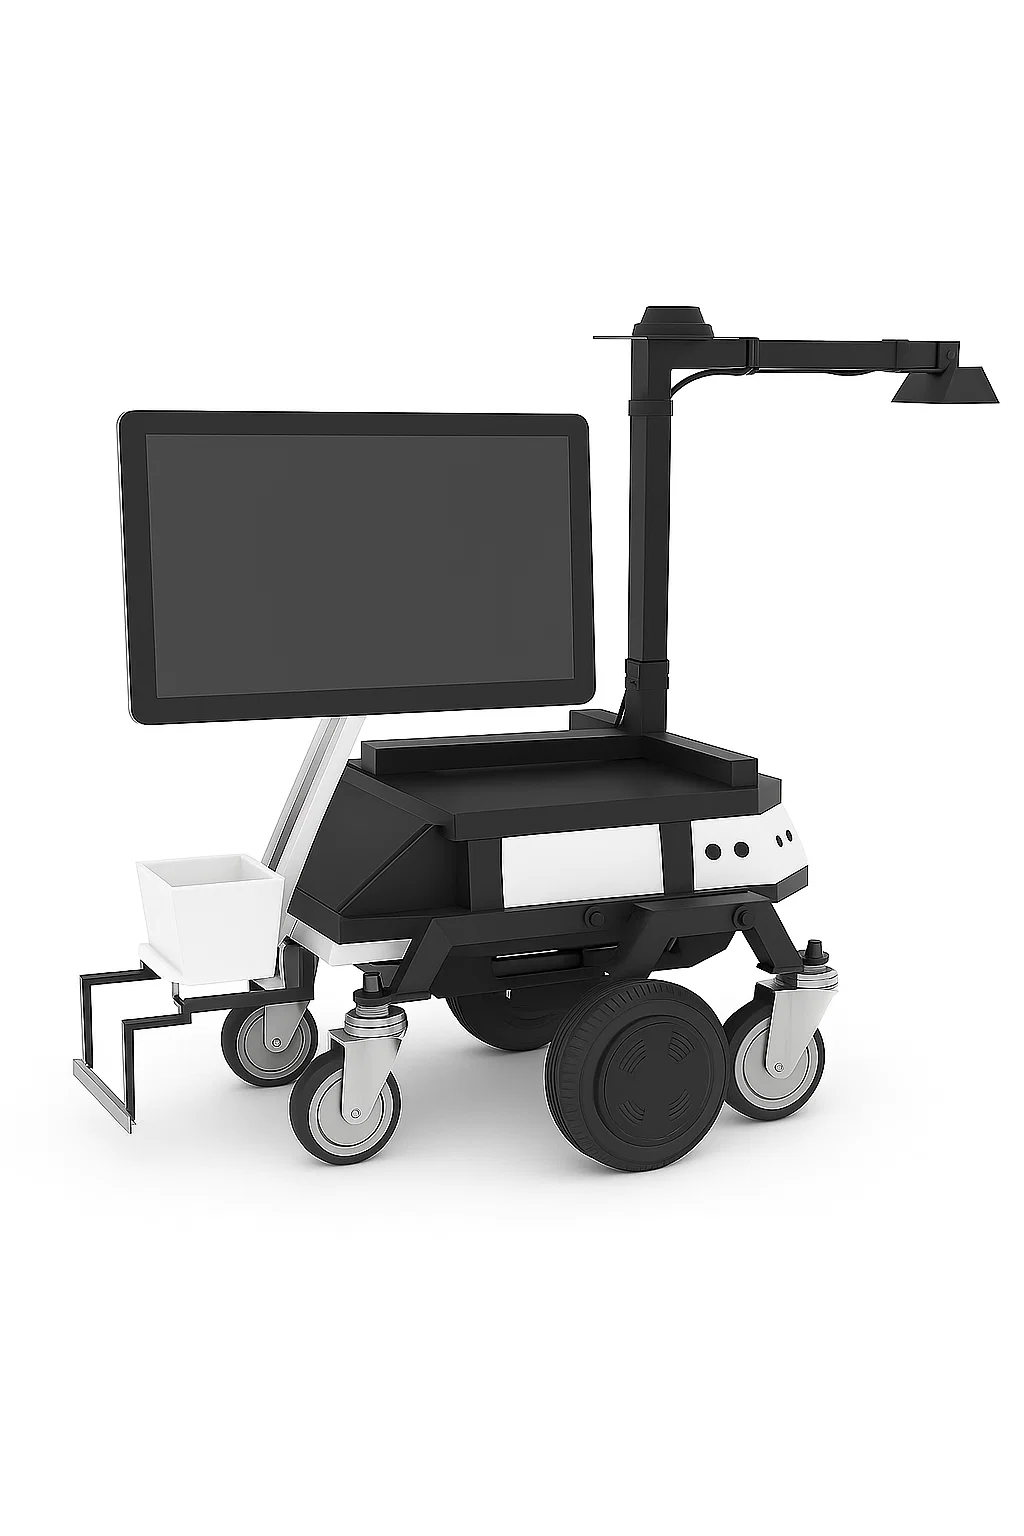
\includegraphics[width=0.7\linewidth]{figures/complete.png}
    \caption{GolfBot System Diagram}
    \label{fig:golfbot_system_diagram}
\end{figure}

\section{Mechanical Design}
\label{sec:mechanical_design}
The mechanical design focuses on the robot's physical construction, ensuring stability, durability, and the proper placement of all sensors and actuators.

\subsection{Chassis and Drivetrain}
\label{ssec:chassis_drivetrain}
The robot's structure is based on a lightweight aluminum chassis with main body dimensions of 500 mm x 360 mm x 115 mm. It uses a differential drive architecture, powered by two wheel hub motors with a wheel diameter of 165 mm and a track width (distance between the motors) of 570 mm. For stability, the drivetrain is supported by rubber caster wheels.

The motor hubs and casters are mounted on two swing arms, which function as a simple suspension system. This allows the robot's main body to remain relatively horizontal while the swing arms absorb minor bumps from uneven terrain. The wheels provide a ground clearance of 100 mm, sufficient for overcoming common obstacles on a golf course fairway. To protect the electronics, all internal components are housed within the main body frame, secured in custom 3D-printed holders and attached with strong, double-sided Velcro to prevent movement during operation.

\subsection{Sensor and Component Mounting}
\label{ssec:sensor_mounting}
To ensure optimal data collection, custom mounts were designed for the primary sensors. An L-shaped 25 mm aluminum box section is mounted on top of the robot's aluminum plate. This structure holds the camera 300 mm in front of the robot and 600 mm above the ground, providing a clear and effective field of view. To protect the camera from direct sunlight and physical impacts, it is housed in a 3D-printed holder featuring a 90-degree hinge, which ensures the camera is positioned orthogonally to the ground.

The same aluminum arm also supports a 2 mm thick stainless steel circular plate that serves as a ground plane for the RTK-GPS rover antenna. Additionally, a stand for the LCD screen, used for the graphical user interface, is mounted on the top frame.

\subsection{Dispensing and Repair Mechanism}
\label{ssec:dispenser_mechanism}
The repair system is mounted at the rear of the robot. A 90-degree folded stainless steel bracket, which was laser-cut for precision, holds the sand dispenser 100 mm above the ground and approximately 900 mm behind the camera's center point. The dispenser itself is 3D-printed from PLA plastic. Its core is a screw auger mechanism, powered by a NEMA 17 stepper motor, which pushes the sand-seed mixture from a hopper out through a nozzle.

Mounted directly behind the dispenser nozzle is a rubber-mounted brush. This brush extends 60 mm from the nozzle and serves to evenly spread the dispensed material, ensuring the divot is filled smoothly. It is attached to the same stainless steel bracket using custom 3D-printed mounts.

\subsection{RTK Base Station Design}
\label{ssec:rtk_base_design}
The ArduSimple RTK system requires a stationary base station to provide correction data to the rover. For this, the base module was placed inside a waterproof plastic box and mounted on a metal pipe. A circular, laser-cut metal plate is fixed to the top of the pipe to hold the RTK base antenna. To ensure signal integrity, this entire assembly is designed to remain stationary, positioned at the highest practical point within the robot's operational area. The base station is powered via a standard USB cable, which can be connected to a laptop or a simple USB wall adapter.

\section{Hardware Architecture}
\label{sec:hardware_architecture}
The hardware architecture describes the electronic components and the flow of data between them. It is designed around a central, powerful controller that processes sensor data and sends commands to the various actuators.

The Arduino Uno plays a critical role as a dedicated low-level controller. It is responsible for managing the NEMA 17 stepper motor (via the A4988 driver) for the dispensing mechanism and reading orientation data from the BNO055 IMU sensor. The Arduino communicates with the main Jetson Orin controller over a serial-over-USB connection. The Rover RTK-GPS module is also connected directly to the main controller via USB, providing it with high-precision location data. This separation of concerns allows the main controller to focus on high-level processing while the Arduino handles real-time actuator control and sensor reading.

% The software architecture of the GolfBot, detailing the ROS 2 nodes, topics, and overall data flow. This section will explain how the different software components (vision, navigation, control) interact.```

\section{Software Architecture}
\label{sec:software_architecture}
The software architecture is designed using the Robot Operating System 2 (ROS 2), which provides a modular framework for concurrent processes. The system's structure is best represented by its ROS 2 computation graph, which shows the active nodes and the topics that connect them.

Figure \ref{fig:ros2_computation_graph} shows the \texttt{rqt\_graph} output from the running GolfBot system. The ellipses represent ROS 2 nodes (the processes), while the rectangular boxes represent topics (the data streams). The arrows indicate the direction of data flow, showing which nodes are publishing and which are subscribing. The following subsections describe the roles of these key components as shown in the graph.

\begin{figure}[h!]
    \centering
    % The user has placed the image in figures/ros2_nodes.png
    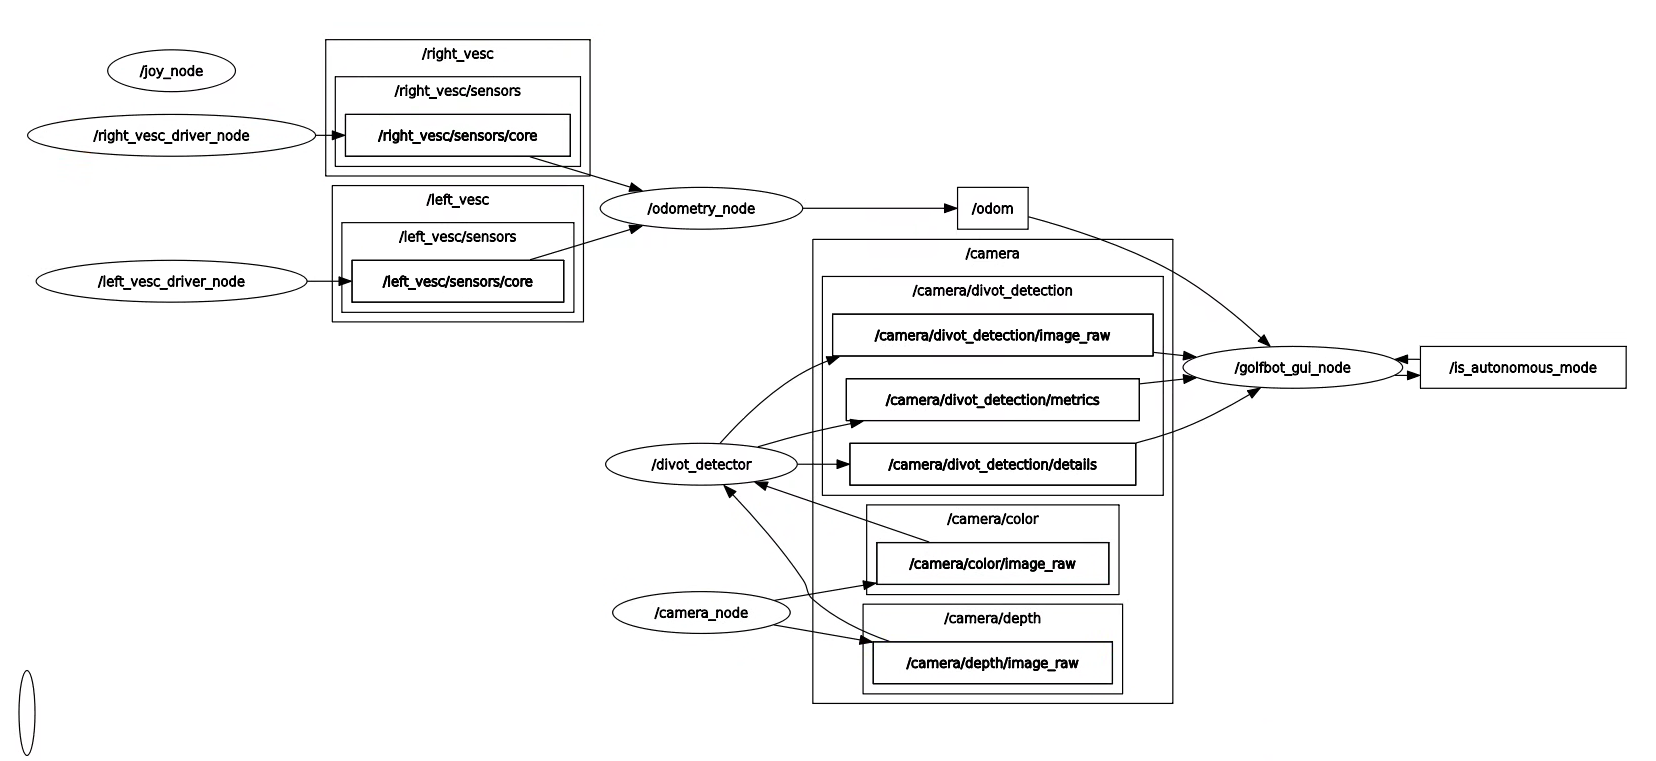
\includegraphics[width=\linewidth]{figures/ros2_nodes.png}
    \caption{ROS 2 computation graph (\texttt{rqt\_graph}) of the running GolfBot system, showing the primary nodes and topics.}
    \label{fig:ros2_computation_graph}
\end{figure}

\subsection{Drivetrain Interface and Odometry}
The core of the robot's mobility and low-level state tracking is handled by a set of dedicated nodes.
\begin{description}
    \item[VESC Driver Nodes (\texttt{/left\_vesc\_driver\_node}, \texttt{/right\_vesc\_driver\_node})] These nodes provide the direct interface to the VESC motor controllers. They are responsible for sending velocity commands to the motors and reading back sensor data, such as motor RPM. They publish their data to the \texttt{/left\_vesc/sensors/core} and \texttt{/right\_vesc/sensors/core} topics respectively.
    \item[Odometry Node (\texttt{/odometry\_node})] This node subscribes to the sensor data from both VESC driver nodes. It uses the wheel speed information to calculate the robot's movement over time. It then publishes this wheel odometry as a \texttt{nav\_msgs/Odometry} message on the \texttt{/odom} topic, providing a basic estimate of the robot's position and orientation.
\end{description}

\subsection{Computer Vision Pipeline}
The vision system is responsible for acquiring images and identifying divots within them.
\begin{description}
    \item[Camera Node (\texttt{/camera\_node})] This node interfaces with the Intel RealSense camera. As shown in the graph, it publishes the raw color and depth image streams to the \texttt{/camera/color/image\_raw} and \texttt{/camera/depth/image\_raw} topics.
    \item[Divot Detector Node (\texttt{/divot\_detector})] This is the primary AI processing node. It subscribes to the \texttt{/camera/color/image\_raw} topic to get live images. It runs the custom-trained YOLO model on these images and publishes its findings to several topics for consumption by other parts of the system:
    \begin{itemize}
        \item \texttt{/camera/divot\_detection/image\_raw}: An annotated video stream with bounding boxes drawn around detected divots, useful for visualization.
        \item \texttt{/camera/divot\_detection/details}: Structured data about the detections (e.g., pixel coordinates, size).
        \item \texttt{/camera/divot\_detection/metrics}: Performance metrics of the detection model.
    \end{itemize}
\end{description}

\subsection{User Interface and Control Logic}
This part of the system provides user control and bridges the gap between perception and action.
\begin{description}
    \item[Joystick Node (\texttt{/joy\_node})] This standard ROS 2 node reads input from the connected Logitech joystick and publishes it to the \texttt{/joy} topic (not shown connected in this graph, but it provides input to the VESC driver nodes for manual control).
    \item[GUI Node (\texttt{/golfbot\_gui\_node})] This node provides a graphical user interface for the operator. It subscribes to the various divot detection topics to display the system's status and the annotated video feed. As seen in the graph, it also interacts with the \texttt{/is\_autonomous\_mode} topic, allowing the operator to switch the robot between manual and autonomous modes.
    \item[Autonomous Node (\texttt{/is\_autonomous\_mode})] This topic (represented as a node in this graph style) acts as a state holder, broadcasting whether the robot should be operating autonomously or under manual control. The GUI node can change this state, and a future mission control node would subscribe to it to know when to begin its work.
\end{description}

\subsection{Navigation and Localization}
This subsystem provides the robot with an accurate sense of its position in the world.
\begin{description}
    \item[GPS Node (\texttt{ublox\_gps\_node})] This is an external ROS 2 package used to interface with the ArduSimple RTK-GPS module. It parses the NMEA data coming from the USB port and publishes it as \texttt{sensor\_msgs/NavSatFix} messages on the \texttt{/fix} topic.
    \item[State Estimation Node (Designed)] In a full implementation, a node like \texttt{robot\_localization} would be used. It would fuse the RTK-GPS data from \texttt{/fix} and the IMU data from \texttt{/imu/data} using an Extended Kalman Filter (EKF) to produce a robust, continuous odometry estimate of the robot's position and orientation.
\end{description}

\subsection{Mechanical and Low-Level Interface}
This component acts as the bridge between the high-level software and the low-level hardware like the dispenser motor and IMU.
\begin{description}
    \item[Arduino Interface Node (\texttt{stepper\_imu\_node.py})] This multi-purpose node handles communication with the Arduino Uno via a serial-over-USB connection. It has two primary functions:
    \begin{enumerate}
        \item It listens for dispenser commands (e.g., from the manual control node or the mission control node) and sends the corresponding serial characters ('R' for Run, 'S' for Stop) to the Arduino.
        \item It continuously reads serial data sent *from* the Arduino, which contains the BNO055 IMU sensor readings, and publishes this data as \texttt{sensor\_msgs/Imu} messages on the \texttt{/imu/data} topic.
    \end{enumerate}
\end{description}